\documentclass[11pt,a4paper]{article}
\usepackage[margin=2.5cm]{geometry}
\usepackage{amsmath,amssymb,amsthm}
\usepackage{booktabs}
\usepackage{graphicx}
\usepackage[hidelinks]{hyperref}
\usepackage{xcolor}

\newcommand{\R}{\mathbb{R}}
\newcommand{\bu}{\mathbf{u}}
\newcommand{\bv}{\mathbf{v}}
\newcommand{\bw}{\mathbf{w}}
\newcommand{\bx}{\mathbf{x}}
\newcommand{\bF}{\mathbf{F}}
\newcommand{\bn}{\mathbf{n}}
\newcommand{\bt}{\mathbf{t}}
\newcommand{\rhat}{\hat{\mathbf{r}}}
\newcommand{\code}[1]{\texttt{#1}}
\newtheorem{proposition}{Proposition}
\newtheorem{lemma}{Lemma}

\title{Numerical methods in \code{dmplex.jl}\\[2pt]
\large Meshes, compatible finite elements and C-grid finite volumes\\
for the rotating shallow-water equations on the sphere}
\author{Oswald Knoth}
\date{Working notes, \today}

\begin{document}
\sloppy
\maketitle

\begin{abstract}
These notes collect the theory behind the discretizations implemented in
\code{dmplex.jl}: the mesh generators and mesh optimizations (bisection,
Voronoi duals, spring dynamics, centroidal Voronoi tessellations, cleanup of
locally refined Delaunay meshes), the compatible finite-element models,
the TRiSK finite-volume scheme on Voronoi meshes with the PV fluxes of
Thuburn--Ringler and Gassmann, a kinetic energy that is both consistent and
energy conserving, and the triangular C grid of ICON. For every scheme the
conservation properties are derived and the known consistency defects are
explained, together with the numerical evidence from Williamson's test case~2
and the Galewsky jet. The staggered kite elements have a separate note
(\code{kite\_shallow\_water.tex}) and are only summarized here.
\end{abstract}

\tableofcontents

%==============================================================================
\section{Equations and test cases}

On the unit sphere with outward normal $\rhat$ the rotating shallow-water
equations in vector-invariant form read
\begin{align}
  \partial_t\bu + q\,\rhat\times\bF + \nabla(K + gh) &= 0, &
  \partial_t h + \nabla\cdot\bF &= 0,
  \label{eq:sw}
\end{align}
with the mass flux $\bF = h\bu$, the kinetic energy $K=\tfrac12|\bu|^2$, the
relative vorticity $\zeta = \rhat\cdot\nabla\times\bu$, the Coriolis parameter
$f = 2\Omega z$ and the potential vorticity $q = (\zeta+f)/h$. Mass $\int h$,
energy
\begin{equation}
  E = \int h K + \tfrac12 g h^2
\end{equation}
and potential enstrophy $\tfrac12\int hq^2$ are conserved. The derivation of
energy conservation is the template for all discretizations below: with
$\partial E/\partial\bu = h\bu = \bF$ and $\partial E/\partial h = K + gh =: B$,
\[
  \dot E = \int \bF\cdot\partial_t\bu + B\,\partial_t h
         = -\int q\,\bF\cdot(\rhat\times\bF) - \int\bF\cdot\nabla B - \int B\,\nabla\cdot\bF = 0,
\]
since $\bF\cdot(\rhat\times\bF) = 0$ pointwise and the gradient is the negative
adjoint of the divergence. A discretization conserves energy if it keeps these
three ingredients: an antisymmetric Coriolis (PV flux) operator, adjoint
gradient and divergence, and a kinetic energy and a mass flux that are linked by
$\partial E_h/\partial\bu = \bF$.

Units: radius $a = 1$, $\Omega = 1$ ($f = 2z$), and in the test cases $g = 1$
(TC2) or the nondimensional gravity of the Galewsky case.

\paragraph{Williamson test case 2 (TC2).} Steady geostrophic solid-body
rotation, $\bu = u_0(-y,x,0)$, $h = 1 - (u_0+u_0^2/2)z^2$, $u_0 = 0.2$, $g = 1$.
The height error after one time unit measures the consistency of the balance
between the Coriolis term and $\nabla(K+gh)$.
The maximum error is the sensitive quantity: an $O(1)$ inconsistency of an operator gives
an $O(1)$ local truncation error of the momentum equation next to the mesh
defects, which shows up as a maximum error that stops converging.

\paragraph{Galewsky jet.} The barotropically unstable mid-latitude jet of
Galewsky et al.\ (2004), $u_{\max} = 80\,\mathrm{m\,s^{-1}}$, mean depth
10\,km, with the height perturbation at $45^\circ$N, integrated for 6 days
without explicit dissipation (unless stated). It tests nonlinear stability:
grid-scale noise, grid imprinting (wavenumber-5 pattern of the icosahedron)
and the vortex roll-up from day 4.

%==============================================================================
\section{Meshes}

All meshes are \code{Plex} objects (DMPlex-like Hasse diagrams of cells,
edges and vertices with cones and supports) on the unit sphere or on a doubly
periodic plane. Cells are oriented counter-clockwise seen from outside.

\subsection{Generators}

\paragraph{Icosahedral triangles} (\code{create\_spherical\_mesh(n)}). The
icosahedron is bisected $n$ times: every triangle is split into four, the
edge midpoints are projected radially onto the sphere. Level $n$ has
$20\cdot4^n$ triangles and $10\cdot4^n+2$ vertices.

\paragraph{Hexagons} (\code{create\_hexagon\_mesh(n)}). The spherical Voronoi
diagram of the icosahedral vertices: the circumcenters of the triangles become
the vertices, every triangle vertex becomes a cell (12 pentagons, the rest
hexagons). The result is an exact Voronoi--Delaunay pair; the generators are
the icosahedral vertices.

\paragraph{Cubed sphere} (\code{create\_cubed\_sphere\_mesh(n)}). Equiangular
gnomonic projection (Sadourny): on every panel the node $(i,j)$ is at the
angles $\alpha_i,\beta_j = -\pi/4 + \pi i/(2n)$, mapped to
$(1,\tan\alpha,\tan\beta)$ and normalized.

\paragraph{HEALPix} (\code{create\_healpix\_mesh(nside)}). The corners of the
$12\,\mathrm{nside}^2$ HEALPix pixels (continuous version of
\code{xyf2loc}), connected by great-circle arcs; the areas are close to but not
exactly equal.

\paragraph{Periodic planes} (\code{create\_periodic\_plane}). Squares or
triangles on a torus.

\paragraph{Grid files} (\code{read\_grid}). ICON triangle grids
(\code{vertex\_of\_cell}) and MPAS Voronoi grids (\code{verticesOnCell}); with
\code{dual=true} the hexagonal dual of an ICON grid (cells around its vertices,
vertices at the triangle circumcenters) or the Delaunay triangles of an MPAS grid
(vertices at the generators, triangles from \code{cellsOnVertex}).

\subsection{Cell centers and orthogonality}

Staggered schemes need a mass point per cell, and C-grid schemes need the
dual edge (through the mass points of two neighbouring cells) to be
orthogonal to the primal edge. \code{cell\_centers} chooses
\begin{itemize}
\item the circumcenter for triangles (the vertex of the Voronoi dual);
\item for Voronoi meshes the generators, recovered from the mesh alone: an edge
  with great-circle normal $\bn$ between cells $i,j$ lies on the perpendicular
  bisector of the generators iff $g_i - g_j\parallel\bn$ and
  $\bn\cdot(g_i+g_j) = 0$. These conditions are linear and homogeneous in all
  generators; their least-squares null vector is found by inverse iteration;
\item the normalized vertex mean otherwise (cubed sphere, HEALPix).
\end{itemize}
The \emph{orthogonality defect} is the largest $|\cos|$ of the angle between
a primal edge and the great circle through the two centers; it is zero for a
Voronoi--Delaunay pair, which the C-grid models require.

\subsection{Defects of bisection meshes}

Plain bisection keeps the shape of the 20 icosahedron faces: across the edges of
the coarser levels the cell shapes jump, and these jumps do not shrink under
refinement. A convenient measure for the triangular C grid is the asymmetry of
the circumcenters about an edge, $|d_{e,l}-d_{e,r}|/d_e$, with $d_{e,l}$,
$d_{e,r}$ the distances of the two circumcenters to the edge and
$d_e = d_{e,l} + d_{e,r}$. It is $0.193$ at every bisection level (ICON's
R02B04/B05 grids, which are optimized: $0.15/0.12$). On the Voronoi side the
TRiSK tangential reconstruction has an $O(1)$ maximum error of $0.11$ on plain
hexagons at all levels (Section~\ref{sec:trisk}).

\subsection{Spring dynamics}
\label{sec:spring}

Following Tomita et al.\ (2002), the edges of the triangle mesh become springs
of natural length $\beta\bar d$; the force on vertex $i$ is
\begin{equation}
  \mathbf f_i = P_i\sum_{j\sim i}(|\bx_j-\bx_i| - \beta\bar d)\,
               \frac{\bx_j-\bx_i}{|\bx_j-\bx_i|},
  \qquad P_i = I - \bx_i\bx_i^T,
\end{equation}
and the damped motion $\bv_i\leftarrow(1-0.05)\bv_i + \Delta t\,\mathbf f_i$,
$\bx_i\leftarrow(\bx_i+\Delta t\,\bv_i)/|\cdot|$ with $\Delta t = 0.3$ (velocities kept
tangential) is iterated to equilibrium. The 12 icosahedron vertices are fixed.
$\bar d$ is fixed by the level, the side of the equilateral triangle with the
mean cell area, $\bar d = \sqrt{4\pi/(5\sqrt3)}/2^n$, so that the equilibrium
does not depend on the starting mesh. The relaxation is applied after every
bisection (multilevel), and it stops when the largest tangential force is below
$10^{-10}\beta\bar d$. For $\beta = 1$ the springs push against each other
weakly; Tomita et al.\ recommend $\beta = 1.2$, and $\beta\ge 1.3$ folds the
mesh over (the code checks the orientation of all triangles). With $\beta=1.2$
the asymmetry drops to $0.10/0.089$ at level 6/7 and the TRiSK tangential
error to $0.014$--$0.018$.

\subsection{Spherical centroidal Voronoi tessellations}

An SCVT is a Voronoi diagram whose generators are the centroids of their
cells (Du, Gunzburger and Ju 2003); the MPAS grids are SCVTs. Lloyd's algorithm
iterates $\bx_i\leftarrow c(V_i)/|c(V_i)|$. The centroid of the spherical
polygon $V_i$ with vertices $c_1,\dots,c_m$ (the circumcenters of the triangles
around $\bx_i$) is exact:
\begin{equation}
  \int_{V_i}\bx\,dA = \frac12\sum_{k=1}^m \theta_k\,
     \frac{c_k\times c_{k+1}}{|c_k\times c_{k+1}|},
  \qquad \theta_k = \angle(c_k,c_{k+1}),
\end{equation}
which follows from Stokes' theorem applied to the constant vector fields, with
$\int_{V}\bx\,dA = \tfrac12\oint \bx\times d\bx$ on the unit sphere and the great-circle
arc contributing $\theta_k$ times its pole.

Plain Lloyd converges slowly (4270 iterations at level 6). The fixed-point
iteration $\bx\leftarrow G(\bx)$ is accelerated by Anderson mixing (type II): with the residuals
$f_k = G(\bx_k)-\bx_k$ and the last $m=16$ differences
$\Delta X$, $\Delta F$ of iterates and residuals,
\[
  \gamma = (\Delta F^T\Delta F + \varepsilon I)^{-1}\Delta F^T f_k,\qquad
  \bx_{k+1} = \bx_k + f_k - (\Delta X + \Delta F)\gamma,
\]
with a small regularization $\varepsilon = 10^{-12}\max\operatorname{diag}$. Level 6
converges in 167 iterations, level 7 in 8\,s. The connectivity is kept, so the
code checks that the triangulation is still Delaunay at the end.

\subsection{Cleanup of locally refined Delaunay meshes}
\label{sec:relax}

The Delaunay dual of the variable-resolution MPAS grid x4.163842 (92--25\,km,
refined around $0^\circ$N $0^\circ$E, 327680 triangles) is far less regular than
an ICON grid: angles up to $94.7^\circ$ (60 triangles above $80^\circ$, 3
obtuse), Voronoi (dual) edges down to 1.2\,km where four MPAS cells nearly meet
in one point, and $d_{e,l}/d_e$ down to $0.003$. \code{relax\_triangles} runs
the spring dynamics with a natural length per edge instead of a global one:
the local size at each vertex (mean adjacent edge chord) is smoothed four times
over the neighbours, and edge $(i,j)$ gets $\beta(s_i+s_j)/2$ with $\beta = 1$.
It is a cleanup, not an optimization: it stops at a force tolerance of $10^{-3}$
of the mean size (4\,s), which removes the nearly right triangles long before
the smooth modes converge. Result: maximum angle $84^\circ$, no obtuse triangle,
shortest dual edge 4.7\,km (four times the time step), edges 15--127\,km
(18--121 before), so the refinement is kept.

\subsection{Kite grids}

Every polygonal cell is split into kites (primal vertex, edge point, center,
edge point); the kites around a primal vertex form a dual cell. The edge point
is the crossing with the dual edge when the mesh has an orthogonal dual. See
the kite note.

%==============================================================================
\section{Compatible finite elements}

\subsection{Spaces}

Elements of any order on triangles and quadrilaterals: \code{Lagrange(k)}
(continuous, Gauss--Lobatto nodes on quads), \code{Discontinuous(k)},
\code{RaviartThomas(k)} (RT on triangles, RTCF on quads: normal components at
Gauss points on the edges plus interior moments), \code{BrezziDouglasMarini(k)} on
quads ($[P_k]^2\oplus\operatorname{span}\{\operatorname{curl}(x^{k+1}y),
\operatorname{curl}(xy^{k+1})\}$, the same normal traces as $\mathrm{RT}_k$ with fewer
dofs) and N\'ed\'elec elements. The reference map is the (bi)linear interpolant
of the cell vertices projected radially onto the sphere. H(div) fields use the
contravariant Piola map $\bv = J\hat\bv/\det J$, so that
$(\nabla\cdot\bv)\eta\,dA = (\hat\nabla\cdot\hat\bv)\hat\eta\,d\xi$ and
$\bv\cdot\bn\,ds = \hat\bv\cdot\hat\nu\,dt$ do not depend on the metric. The surface
normal is $\rhat = J_1\times J_2/|J_1\times J_2|$.

The degrees of freedom are attached to mesh points by a \code{Section};
closures give global indices with orientation signs, so normal continuity of
H(div) and continuity of $H^1$ spaces hold exactly.

\paragraph{Mass solvers.} \code{mass\_solver(V)} assembles and caches the mass
matrix of a space: diagonal when lumped at the element nodes (Gauss--Lobatto or
Gauss--Radau tensor nodes), block diagonal for broken spaces (stored inverses
of the blocks), otherwise a sparse Cholesky factorization. In parallel the
coupled matrices are solved by gathering (\code{GatheredMassSolver}, replicated
Cholesky) or with cuDSS on GPUs.

\subsection{Linear shallow water}

With $\bu\in\mathrm{RT}_k$, $h\in\mathrm{DG}_k$,
\begin{equation}
  M_u\dot\bu = -C\bu + g D^Th, \qquad M_h\dot h = -H D\bu,\qquad
  D_{ij} = \int\psi_i\nabla\cdot\bv_j,\quad C_{ij} = \int f\,\bv_i\cdot(\rhat\times\bv_j).
\end{equation}
$C$ is antisymmetric, so the energy $\tfrac12H\bu^TM_u\bu + \tfrac12 g h^TM_hh$ is
conserved exactly; mass is conserved since $\nabla\cdot\mathrm{RT}_k\subset\mathrm{DG}_k$.
Since $\nabla\cdot$ maps $\mathrm{RT}_k$ onto $\mathrm{DG}_k$ there are no spurious
pressure modes and the steady geostrophic modes are represented (Cotter and
Shipton 2012).

\subsection{Nonlinear shallow water}

The scheme of McRae and Cotter (2014), as in Gusto: $\bu,\bF\in\mathrm{RT}_k$,
$h,K\in\mathrm{DG}_k$, $\omega\in\mathrm{CG}_{k+1}$,
\begin{align}
  \int\gamma\,\omega &= -\int\bu\cdot(\rhat\times\nabla\gamma) + \int\gamma f,&
  \int\bw\cdot\bF &= \int\bw\cdot h\bu,&
  \int\phi\,K &= \int\phi\,\tfrac12|\bu|^2,\\
  \int\bw\cdot\dot\bu &= -\int\bw\cdot\Bigl(\frac{\omega}{h}\rhat\times\bF\Bigr)
     + \int(\nabla\cdot\bw)(gh + K),\\
  \int\phi\,\dot h &= -\int\phi\,\nabla\cdot\bF.
\end{align}
\begin{proposition}
The semi-discretization conserves mass and $E_h = \int\tfrac12 h|\bu|^2 + \tfrac12gh^2$.
\end{proposition}
\begin{proof}
With the same quadrature in $E_h$ and the right-hand sides,
$\partial E_h/\partial\bu = M_u\bF$ (definition of $\bF$) and
$\partial E_h/\partial h = M_h(K+gh)$ (definition of $K$). Testing the momentum
equation with $\bw = \bF$ removes the PV flux term ($(\rhat\times\bF)\cdot\bF = 0$
pointwise for any $q$), and the remaining terms cancel with the continuity
equation tested with $\phi = K+gh$.
\end{proof}
The vorticity is diagnosed with the constant mass matrix of $\mathrm{CG}_{k+1}$,
so all mass matrices are factorized once. The nonlinear terms are kernels over
the cells on bases tabulated once (\code{CellTables}).

\subsection{Staggered kite elements}

Summary of the kite note: the height lives in \code{KiteRadau(p)} ($Q_p$ on the
kites with Gauss--Radau nodes that include the center side: continuous inside a
primal cell, broken across primal edges, diagonal lumped mass); the velocity in
\code{KiteBrokenRT(k)} (normal continuity across the half edges inside a dual
cell, broken across the dual-cell boundaries, block-diagonal mass per dual
cell), \code{KiteBrokenBDM(k)} or \code{KiteDualRadau(p)} (Wess, Kapidani,
Codecasa and Sch\"oberl 2024); vorticity in CG$_{k+1}$ with lumped mass. The
divergence $D$ and the gradient $G$ are defined with face terms on the
respective broken edges and satisfy $G = -D^T$ exactly. The conservative nonlinear
variant projects $\bF = \Pi_{V_u}(h\bu)$ and conserves mass and energy as in the
proposition above; all mass matrices stay (block) diagonal, so the scheme is
explicit and local.

%==============================================================================
\section{Finite-volume upwind advection}

\code{compute\_advection\_rhs!} is the first-order upwind scheme for a
cell-wise constant tracer $C$ with given normal velocities $U_e$:
\[
  A_i\dot C_i = -\sum_{e\in i} n_{e,i}\,l_e\,U_e\,C_{\mathrm{up}(e)},
\]
with $C_{\mathrm{up}}$ the value of the cell upstream of edge $e$. It conserves
$\sum A_iC_i$ and is monotone under the CFL condition.

%==============================================================================
\section{C-grid finite volumes on Voronoi meshes: TRiSK}
\label{sec:trisk}

\subsection{Geometry}

\code{TRiSKGrid} describes a Voronoi--Delaunay pair: primal cells $i$ (Voronoi
polygons) with mass points at the generators $g_i$, dual cells $v$ (the
triangles of three generators around a mesh vertex $x_v$), and edges $e$ with the
normal $\bn_e$ from the left cell to the right cell. Per edge: the primal length
$l_e$ (between its vertices), the dual length $d_e$ (between the generators),
the edge point $m_e$ where both cross, and the distances $d_{e,i}$ of the generators to $m_e$.
Kites $K_{i,v}$ (cell $i$ $\cap$ dual cell $v$) are pairs of spherical triangles
$(g_i, m_e, x_v)$; the cell areas $A_i$ and dual areas $A_v$ are their sums, so
the kite fractions $R_{i,v} = K_{i,v}/A_i$ add up to one in every cell, which is
what the TRiSK weights need.

On Delaunay meshes with obtuse triangles the circumcenter lies beyond an edge.
All distances and kites are then \emph{signed}: $d_{e,i}<0$ for a generator beyond
the edge, and spherical triangles get the signed area
\begin{equation}
  A(a,b,c) = 2\operatorname{atan2}\bigl(a\cdot(b\times c),\ 1 + a\cdot b + b\cdot c + c\cdot a\bigr),
\end{equation}
which is negative for clockwise triangles (Van Oosterom--Strackee). With signed
kites the areas are exact for any Delaunay mesh.

\subsection{Operators}

With $n_{e,i} = \pm1$ (outward) and $t_{e,v}=\pm1$ (counter-clockwise around $v$):
\begin{align}
  (D\bF)_i &= \frac1{A_i}\sum_{e\in i} n_{e,i}\,l_e F_e, &
  (G\phi)_e &= \frac{\phi_r - \phi_l}{d_e}, &
  \zeta_v &= \frac1{A_v}\sum_{e\in v} t_{e,v}\,d_e u_e.
\end{align}
With the inner products $\langle a,b\rangle_c = \sum_i A_ia_ib_i$ on cells and
$\langle u,w\rangle_e = \sum_e l_ed_e u_ew_e$ on edges,
$\langle D F,\phi\rangle_c = -\langle F, G\phi\rangle_e$ exactly (summation by parts), and
the discrete identities $\zeta(G\phi) = 0$, $D(\text{skew gradient}) = 0$ hold
as in the continuum.

\paragraph{TRiSK weights.} The tangential velocity at edge $e$ is reconstructed
from the edges of its two cells (Thuburn et al.\ 2009),
\begin{equation}
  v_e = \frac1{d_e}\sum_{e'} w_{e,e'}\,l_{e'}u_{e'},\qquad
  w_{e,e'} = n_{e,i}\,n_{e',i}\Bigl(\tfrac12 - \sum_{v} R_{i,v}\Bigr),
\end{equation}
with the sum over the corners of cell $i$ passed when walking counter-clockwise from
$e$ to $e'$. The weights are antisymmetric, $w_{e,e'} = -w_{e',e}$, and the dual divergence of the
perpendicular fluxes equals the kite average of the primal divergence, which
makes the linear geostrophic modes steady.

\subsection{The nonlinear TRiSK scheme}

Following Ringler et al.\ (2010), with $F_e = h_eu_e$:
\begin{align}
  h_v &= \frac1{A_v}\sum_i K_{i,v}h_i, & q_v &= \frac{\zeta_v + f_v}{h_v}, &
  q_e &= \tfrac12(q_{v_1}+q_{v_2}),\\
  \partial_tu_e &= \frac1{d_e}\sum_{e'}w_{e,e'}\,l_{e'}F_{e'}\,\frac{q_e+q_{e'}}2
     - (G B)_e, & B_i &= K_i + gh_i, &
  \partial_th_i &= -(DF)_i.
\end{align}
\begin{proposition}
\label{prop:trisk}
Let the kinetic energy be any quadratic form $K_i = \sum_e c_{i,e}u_e^2$ and the
edge height
\begin{equation}
  h_e = \frac{2}{l_ed_e}\sum_i A_i\,c_{i,e}\,h_i .
  \label{eq:he}
\end{equation}
Then the scheme conserves mass and the energy $E = \sum_iA_i(h_iK_i + \tfrac12gh_i^2)$.
\end{proposition}
\begin{proof}
$\partial E/\partial u_e = 2u_e\sum_iA_ih_ic_{i,e} = l_ed_e\,h_eu_e = l_ed_eF_e$ and
$\partial E/\partial h_i = A_iB_i$. Hence
\[
  \dot E = \sum_e l_ed_eF_e\,\partial_tu_e + \sum_iA_iB_i\,\partial_th_i
  = \sum_{e,e'} l_eF_e\,w_{e,e'}l_{e'}F_{e'}\tfrac{q_e+q_{e'}}2
    - \langle F,GB\rangle_e - \langle DF,B\rangle_c .
\]
The double sum vanishes because $w_{e,e'}\frac{q_e+q_{e'}}2$ is antisymmetric in
$(e,e')$ and the rest is symmetric; the last two terms cancel by summation by parts.
Mass: $\sum_iA_i(DF)_i = 0$ since every edge appears twice with opposite signs.
\end{proof}
The PV flux conserves energy for \emph{any} edge PV, the condition~\eqref{eq:he}
links only $K$ and $h_e$. For the cell kinetic energy (ICON's \code{e\_inn\_c})
\begin{equation}
  K_i^{\mathrm{cell}} = \frac1{A_i}\sum_{e\in i}\tfrac12\,l_ed_{e,i}\,u_e^2
  \label{eq:Kcell}
\end{equation}
\eqref{eq:he} gives the distance-weighted mean $h_e = (d_{e,l}h_l + d_{e,r}h_r)/d_e$.

\subsection{Gassmann's PV flux}

\code{pv\_flux = :gassmann} replaces the TRiSK reconstruction by that of Gassmann
(2013) with the PV usage of Gassmann (2018), as in ICON-IAP
(\code{i\_cori\_method = 1}): the tangential flux at $e$ is reconstructed from
the twelve edges of the two vertices of $e$ (the inner edges) and of their outer
vertices,
\[
  \sum_k W_{k,e}\,F_{e_k}\,q_{p(k)} \approx q\,\bF\cdot(\rhat\times\bn_e),
\]
with rhombus PV $q_e = (\zeta_e + f_e)/h_e$,
$\zeta_e = (A_{v_1}\zeta_{v_1}+A_{v_2}\zeta_{v_2})/(A_{v_1}+A_{v_2})$ (likewise $h_e$).
An outer edge carries the PV of its inner edge, an inner edge that of the third
edge of the shared vertex. The weights combine the triangle of the vertex and
the three rhombi around it; with the metric $\bn_k\cdot(\rhat\times\bn_e)$ taken
at the midpoint of both edge points, $l_ed_eW_{k,e} = -l_{e'}d_{e'}W_{j,e'}$ for the
pair with the same PV, so the term does no work. Unlike TRiSK it is consistent on
the hexagon mesh: tangential maximum error $0.015\to0.0016$ from hexagon 3 to 6
(TRiSK $0.12$); TC2 L2 errors are 2--4 times smaller. Without dissipation its PV
usage lets grid-scale vorticity grow in the Galewsky jet from day~3;
\code{:gassmann\_mean} uses the same weights with the mean $(q_e+q_{e'})/2$ and stays
smooth (three ghost rings).

\subsection{Consistency of the reconstruction on optimized meshes}

\begin{table}[ht]
\centering
\begin{tabular}{lccc}
\toprule
max error of $v_e$ (solid body) & level 5 & level 6 & level 7\\
\midrule
plain bisection & 0.11 & 0.11 & 0.11\\
spring, $\beta=1.2$ & 0.014 & 0.016 & 0.018\\
SCVT & 0.0071 & 0.0072 & 0.0073\\
\bottomrule
\end{tabular}
\caption{TRiSK tangential reconstruction: inconsistent on every grid, as found
by Peixoto (2016), but an order of magnitude better on optimized grids.}
\end{table}
On spring hexagons the TC2 L2 error is 3--4.5 times and the maximum error 3--5
times smaller than on plain ones (hexagon 4--6). On SCVT hexagons TC2 is not
better than on spring ones: the maximum error is dominated by the kinetic energy.

%==============================================================================
\section{A consistent, energy-conserving kinetic energy}
\label{sec:kinetic}

\subsection{Why the cell kinetic energy is inconsistent}

For a constant tangent vector $\bu$ with $u_e = \bu\cdot\bn_e$,
\eqref{eq:Kcell} gives $K_i = \tfrac12\bu^TT_i\bu$ with the tensor
\[
  T_i = \frac1{A_i}\sum_{e\in i} l_ed_{e,i}\,\bn_e\bn_e^T,
\]
and consistency requires $T_i = I$ on the tangent plane.
\begin{lemma}
\label{lem:polygon}
Let $P$ be a planar polygon with area $A$, sides $s_e$ of length $|s_e|$, outward
normals $\bn_e$ and midpoints $m_e$, and let $c$ be any point. Then
\begin{equation}
  \sum_e |s_e|\,\bn_e(m_e - c)^T = A\,I .
\end{equation}
If $p_e$ is the foot of the perpendicular from $c$ to the line of $s_e$,
$h_e = \bn_e\cdot(p_e - c)$ its signed distance and $m_e - p_e = \tau_e\bt_e$, then
\begin{equation}
  \sum_e |s_e|\,h_e\,\bn_e\bn_e^T = A\,I - \sum_e|s_e|\,\tau_e\,\bn_e\bt_e^T .
\end{equation}
\end{lemma}
\begin{proof}
By the divergence theorem $\int_P\nabla\bx\,dA = \oint\bn\,\bx^T\,ds$; the left
side is $AI$, the right side $\sum_e|s_e|\bn_em_e^T$ because $\bx$ is linear on
each side. Subtract $\sum_e|s_e|\bn_e c^T = 0$. The second identity follows from
$m_e - c = h_e\bn_e + \tau_e\bt_e$.
\end{proof}
For a Voronoi cell, $d_{e,i}$ is the distance from $g_i$ to the edge point $m_e$,
which \emph{is} the foot of the perpendicular (the dual edge is orthogonal to the
primal edge), but not the midpoint of the primal edge. So
$T_i = I - \frac1{A_i}\sum_e l_e\tau_e\bn_e\bt_e^T$, where $\tau_e$ is the offset of
the edge point from the primal edge midpoint. This offset is a fixed fraction
of the cell size on irregular meshes and does not shrink with refinement: the
error of $K^{\mathrm{cell}}$ is $O(1)$ and that of $\nabla K$ is $O(1/h)$. Next
to the pentagons it is 2\,\% on SCVTs and 1.1--1.5\,\% on spring meshes at every
resolution, and the momentum residual of the balanced TC2 state doubles with
every level and sits next to a pentagon.

\subsection{The vertex kinetic energy}

For a dual triangle with its circumcenter $x_v$, the foot of the perpendicular from
$x_v$ to each side \emph{is} the midpoint of that side: $\tau_e = 0$ in
Lemma~\ref{lem:polygon}. The sides are the dual edges ($|s_e| = d_e$) and the
distances are $l_{e,v}$, the length of the part of the primal edge from $x_v$ to
$m_e$. With the areas
\begin{equation}
  A_{e,v} = \tfrac12 l_{e,v}d_e = \text{area of the triangle } (g_l, g_r, x_v),
\end{equation}
Lemma~\ref{lem:polygon} gives $\sum_{e\in v}A_{e,v}\bn_e\bn_e^T = \tfrac12A_vI$
(exactly in the plane, up to $O(h^2)$ curvature terms on the sphere), so
\begin{equation}
  K_v = \frac1{A_v}\sum_{e\in v}A_{e,v}\,u_e^2
  \label{eq:Kv}
\end{equation}
is consistent on \emph{any} Delaunay triangle. The cell value is the kite average,
$K_i^{\mathrm{vertex}} = \sum_v R_{i,v}K_v$, as in Ringler et al.\ (2010) and
Skamarock et al.\ (2012). Two details matter:
\begin{itemize}
\item MPAS uses $l_ed_e/4$ instead of $A_{e,v}$, which assumes that $x_v$ lies at
  the midpoint of the primal edge, i.e.\ it reintroduces an offset like $\tau_e$. On
  spring hexagon 5 that version has a 3.1\,\% error, worse than the cell kinetic energy
  (1.4\,\%).
\item On an obtuse dual triangle the circumcenter lies beyond the long side and
  $A_{e,v}$ for that side is negative. The sign must come from the topology, not
  from the position of $x_v$: in the counter-clockwise left cell of $e$, crossing an
  edge that ends at $v$ turns counter-clockwise around $v$, and then
  $A_{e,v} = +A(g_l,g_r,x_v)$, otherwise $-A(g_l,g_r,x_v)$. With this sign
  $\sum_eA_{e,v} = A_v$ to round-off also for non-convex dual polygons
  (\code{vertex\_edge\_areas}).
\end{itemize}

\subsection{Mixture and energy conservation}

\code{TRiSKShallowWater(\dots; kinetic\_energy)} uses
\begin{equation}
  K_i = \alpha K_i^{\mathrm{cell}} + (1-\alpha)\sum_v R_{i,v}K_v,
  \qquad \alpha = 1\ (\code{:cell}),\ \tfrac38\ (\code{:mixed}),\ 0\ (\code{:vertex}).
\end{equation}
Its coefficients are
$A_ic_{i,e} = \tfrac\alpha2l_ed_{e,i} + (1-\alpha)\sum_{v\in e}K_{i,v}A_{e,v}/A_v$, so
\eqref{eq:he} gives the energy-conserving edge height
\begin{equation}
  h_e = \alpha\,\frac{d_{e,l}h_l + d_{e,r}h_r}{d_e}
      + (1-\alpha)\,\frac{2\,(A_{e,v_1}h_{v_1} + A_{e,v_2}h_{v_2})}{l_ed_e},
  \qquad h_v = \frac1{A_v}\sum_iK_{i,v}h_i,
\end{equation}
the vertex part being the analogue of the distance-weighted mean along the primal
edge (the weights add up to one up to curvature). The vertex heights $h_v$ are
the ones the PV needs anyway. By Proposition~\ref{prop:trisk} mass and energy are
conserved for every $\alpha$. The stencil of $K$ at a ghost cell next to an owned
edge reaches the edges of the cells around its vertices, which are inside the two
vertex rings of ghost cells the PV flux already needs; 1 and 3 MPI ranks give
bitwise identical results.

\subsection{Results}

\begin{table}[ht]
\centering
\begin{tabular}{llccc}
\toprule
mesh & $K$ & hexagon 4 & hexagon 5 & hexagon 6\\
\midrule
\multicolumn{5}{l}{\emph{error of $K$ for a solid-body rotation, relative}}\\
spring & cell & 1.5\,\% & 1.4\,\% & 1.25\,\%\\
spring & vertex & 0.60\,\% & 0.27\,\% & 0.13\,\%\\
SCVT & cell & 2.0\,\% & 2.0\,\% & 2.0\,\%\\
SCVT & vertex & 0.50\,\% & 0.21\,\% & 0.09\,\%\\
plain & cell & 5.9\,\% & 5.8\,\% & 5.8\,\%\\
plain & vertex & 0.71\,\% & 0.33\,\% & 0.16\,\%\\
\midrule
\multicolumn{5}{l}{\emph{TC2, maximum height error at $t=1$}}\\
spring & cell & 4.9e-4 & 3.2e-4 & 2.6e-4\\
spring & mixed & 2.6e-4 & 1.4e-4 & 1.0e-4\\
spring & vertex & 1.8e-4 & 7.2e-5 & 3.8e-5\\
SCVT & cell & 6.3e-4 & 4.2e-4 & 3.5e-4\\
SCVT & vertex & 2.7e-4 & 9.9e-5 & 4.3e-5\\
\midrule
\multicolumn{5}{l}{\emph{TC2, L2 height error at $t=1$}}\\
spring & cell & 1.4e-4 & 3.9e-5 & 1.2e-5\\
spring & vertex & 9.0e-5 & 2.2e-5 & 5.7e-6\\
\bottomrule
\end{tabular}
\caption{Cell versus vertex kinetic energy (TRiSK PV flux). The vertex $K$
converges at first order and lets the TC2 maximum error converge again
(about first order, the remaining error is the TRiSK reconstruction); with the
cell $K$ it stalls. Energy is conserved to round-off with all variants
(relative change below $10^{-14}$ over one time unit on spring hexagon 6 with $\alpha = 0$).}
\end{table}

The Galewsky jet runs stably for 6 days with all three variants on plain and
spring hexagon 6, and with the vertex $K$ on SCVT hexagon 6 and spring hexagon 7:
energy conserved to $5\cdot10^{-10}$ or better, the vorticity extremes and the roll-up
unchanged, no grid-scale noise (the known risk of a pure vertex kinetic energy, the
reason for Skamarock's mixture). The vertex part costs 25--35\,\% more time per
step. The default stays \code{:cell}; the results argue for \code{:vertex}.

\begin{figure}[ht]
\centering
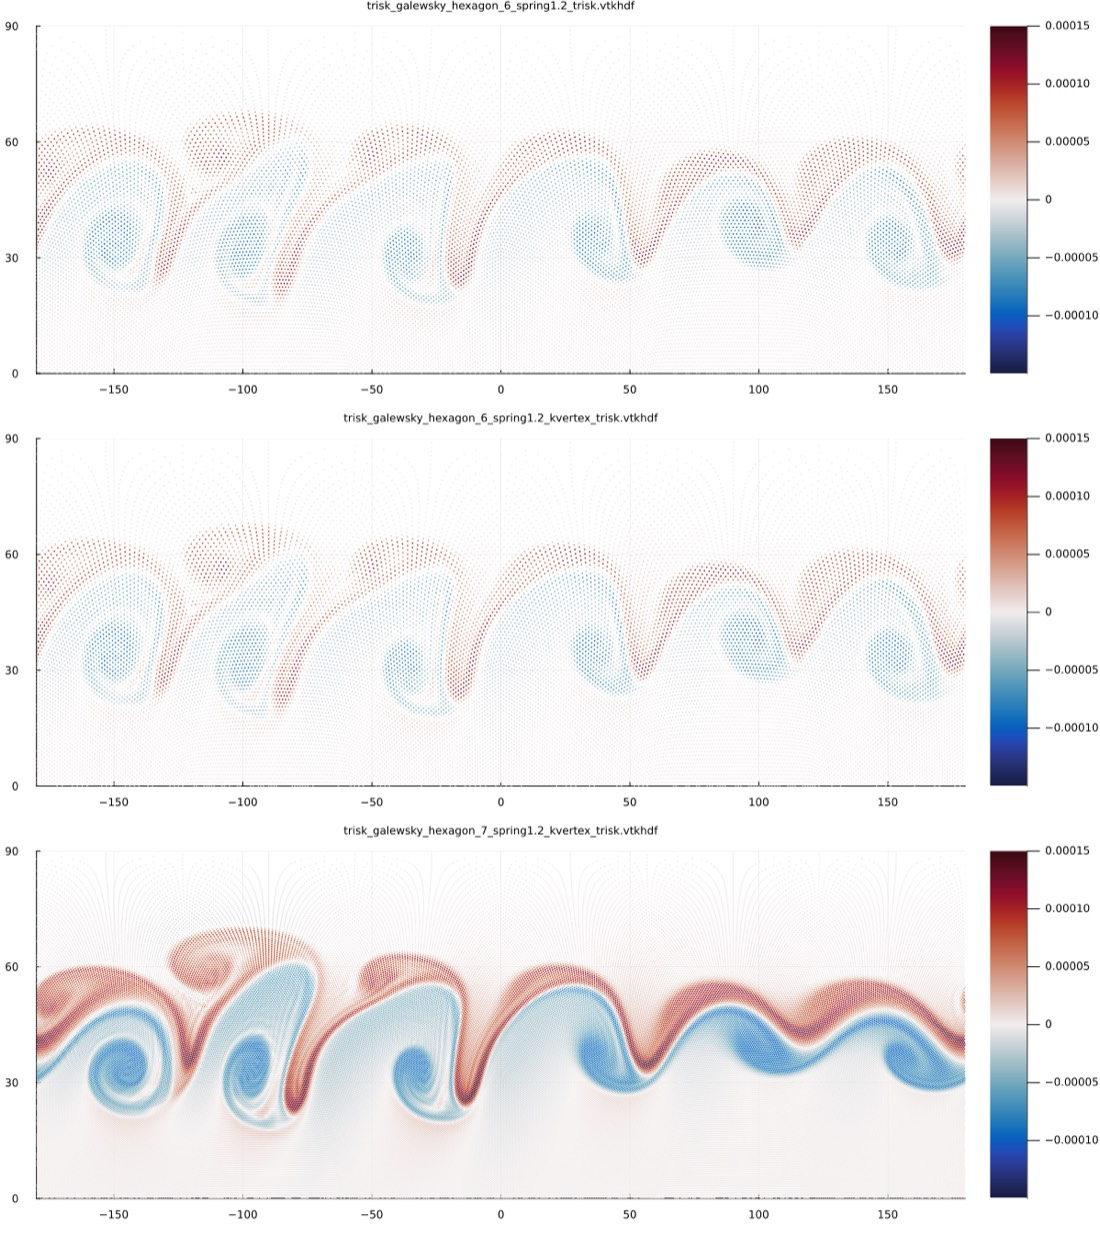
\includegraphics[width=0.85\textwidth]{figures/kinetic_galewsky.jpg}
\caption{Galewsky jet, relative vorticity at day 6 (1/s): spring hexagon 6 with
the cell (top) and the vertex kinetic energy (middle), spring hexagon 7 with the
vertex kinetic energy (bottom).}
\end{figure}

%==============================================================================
\section{The triangular C grid of ICON}
\label{sec:icon}

\subsection{Operators}

\code{ICONShallowWater} ports the horizontal operators of ICON's nonhydrostatic
core (\code{velocity\_tendencies}, ICON 2024.07) to the shallow-water equations:
normal velocities at the edge midpoints, heights at the triangle circumcenters,
vorticity at the vertices (the hexagonal dual cells). It reuses \code{TRiSKGrid}
with the roles of the meshes exchanged.
\begin{align}
  v_e &= \sum_{k=1}^4 c_{e,k}u_k, \qquad
  K_e = \tfrac12(u_e^2+v_e^2),\qquad K_i = \sum_e b_{i,e}K_e,\qquad
  \zeta_e = \tfrac12(\zeta_{v_1}+\zeta_{v_2}),\\
  \partial_tu_e &= (f_e+\zeta_e)v_e - \bigl[K_e(a_1-a_2) + a_2K_r - a_1K_l\bigr]
                   - g\frac{h_r-h_l}{d_e},\\
  \partial_th_i &= -\frac1{A_i}\sum_e n_{e,i}l_eh_eu_e, \qquad
     h_e = \frac{d_{e,r}h_l + d_{e,l}h_r}{d_e},
\end{align}
with the vector-RBF tangential velocity $v_e$, the bilinear edge-to-cell weights
$b_{i,e}$ (\code{e\_bln\_c\_s}), the linear interpolation $h_e$ to the edge midpoint
(\code{c\_lin\_e}) and $a_1 = d_{e,r}/(d_{e,l}d_e)$, $a_2 = d_{e,l}/(d_{e,r}d_e)$
(\code{coeff\_gradekin}).
The RBF coefficients of edge $e$ use the other four edges of its two triangles,
the kernel $\varphi(r) = (1+(r/0.5)^2)^{-1/2}$ times $\bn_i\cdot\bn_j$, normalized
so that constant vectors along $\rhat\times\bn_e$ are reproduced. The bilinear
weights satisfy $\sum_kb_k = 1$ and $\sum_kb_kx_k = 0$ in the tangent plane, so linear
fields are not aliased into a checkerboard. Mass is conserved; energy is not
(the RBF reconstruction is not part of an antisymmetric operator).

\subsection{The kinetic-energy gradient on irregular triangles}

The gradient of ICON is the derivative of the parabola through $(-d_{e,l},K_l)$,
$(0,K_e)$, $(d_{e,r},K_r)$ at the edge: second order, but it contains the edge's
own $K_e$ (with the RBF $v_e^2$) with the weight
\[
  a_1 - a_2 = \frac{d_{e,r}^2 - d_{e,l}^2}{d_{e,l}d_{e,r}d_e},
\]
which vanishes only for symmetric circumcenters and grows like $1/d_{e,l}$ when
a circumcenter approaches the edge. On the symmetric ICON grids it is harmless;
on plain bisection meshes (asymmetry 0.19 at every level) it couples $K_e$, which
contains the tangential velocity, into the momentum equation in a
Hollingsworth-like way: the Galewsky jet blows up on triangle 5/6/7 before day
3/2/1, earlier on finer meshes, independent of time step and damping, and the
TC2 L2 error stalls ($1.9\cdot10^{-5}$, $7.0\cdot10^{-6}$, $3.9\cdot10^{-6}$ for
triangle 4/5/6). With the centered gradient $(K_r-K_l)/d_e$
(\code{kinetic\_gradient = :centered}, $a_1=a_2=1/d_e$) triangle 5 stays stable.
On spring meshes ($\beta = 1.2$) the original scheme works: TC2 converges at
second order ($2.3\cdot10^{-5}$, $5.6\cdot10^{-6}$, $1.4\cdot10^{-6}$) and the
Galewsky jet is stable on triangle 5, 6 and 7 (energy within $3\cdot10^{-7}$
on triangle 7, roll-up as on R02B05).

ICON averages $K_e$ to the cells with the bilinear weights. A cell kinetic energy of
the form~\eqref{eq:Kcell} on the triangles, $\sum_e\tfrac12l_ed_{e,i}u_e^2/A_i$ with $l_e$ the
triangle side and $d_{e,i}$ the distance of the circumcenter, would be consistent by
Lemma~\ref{lem:polygon}, since the circumcenter projects onto the side midpoints;
together with~\eqref{eq:he} it would make the mass flux part energy consistent, but
the RBF Coriolis term still is not.

\subsection{Divergence damping}

The triangular C grid has divergence and checkerboard modes that are not
controlled without dissipation; ICON adds fourth-order divergence damping
$-\nu_4\nabla(\nabla\cdot(\nabla(\nabla\cdot\bu)))$ with
$\nu_4 = 0.0025\,\bar A^2/\Delta t$ (\code{divdamp\_fac}, mean cell area $\bar A$).
On locally refined meshes the time step is set by the smallest cells, and a uniform
$\nu_4$ from the mean area exceeds the explicit stability limit there, which
scales with $A_{\min}^2/\Delta t$. \code{divergence\_damping} therefore
accepts one value per edge; the examples use
$\nu_{4,e} = 0.0025\,A_e^2/\Delta t$ with $A_e$ the mean area of the two cells of $e$.

\subsection{Locally refined MPAS meshes}

On the raw Delaunay dual of x4.163842 (Section~\ref{sec:relax}) TC2 with
\code{coeff\_gradekin} blows up before $t = 0.25$, both on the raw and on the
cleaned mesh. With the centered gradient it is stable: on the raw dual the L2
error is $1.2\cdot10^{-6}$, but the maximum error grows to $5.9\cdot10^{-5}$ at $t=1$; on the
cleaned mesh the L2 error is $1.2\cdot10^{-6}$, the maximum $1.3\cdot10^{-5}$, energy
$-1.5\cdot10^{-8}$. The Galewsky jet on the cleaned mesh (6 days, $\Delta t = 5.8$\,s,
89201 RK4 steps, 36\,min on a laptop CPU) is NaN before day 0.5 with uniform
damping and stable with the local damping: energy within $1.5\cdot10^{-6}$, potential
enstrophy $-1.6\cdot10^{-4}$, $|\zeta|\le1.44\cdot10^{-4}\,\mathrm{s}^{-1}$, the expected
roll-up without imprint of the refinement, close to R02B06.

\begin{figure}[ht]
\centering
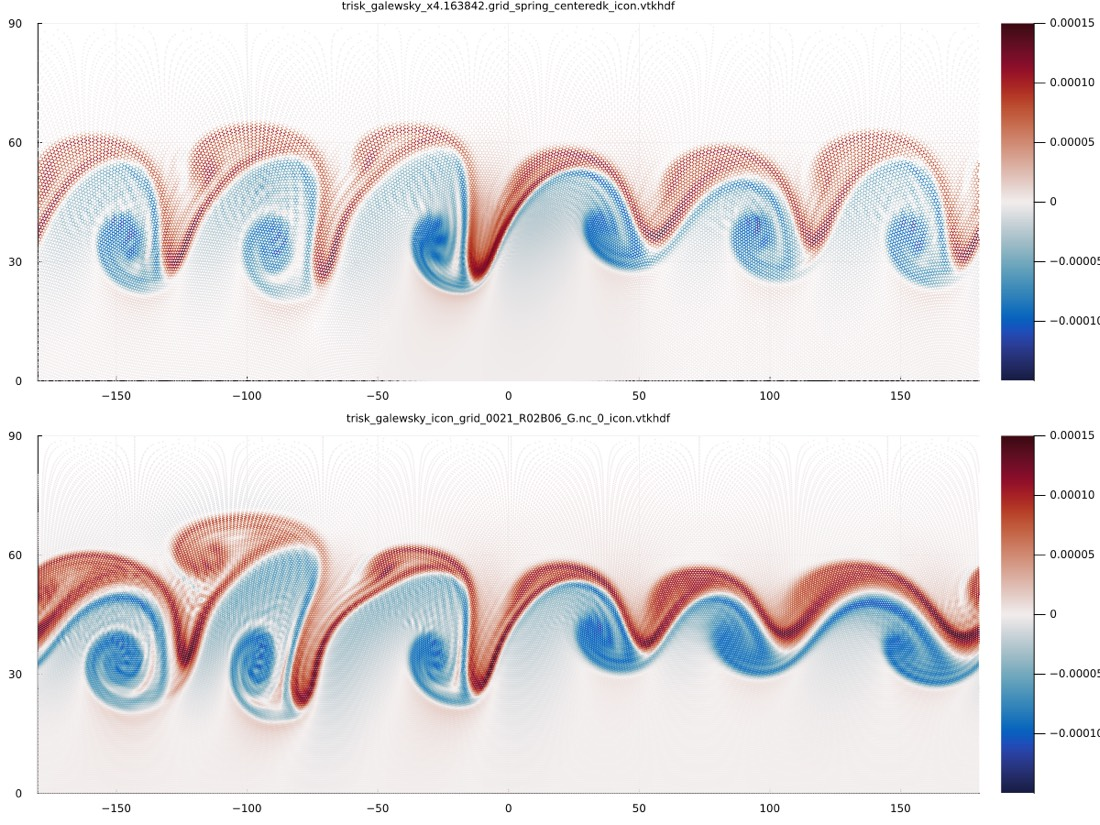
\includegraphics[width=0.85\textwidth]{figures/mpas_vr_galewsky.jpg}
\caption{Galewsky jet, relative vorticity at day 6 with the ICON model: on the
cleaned Delaunay dual of the locally refined MPAS grid x4.163842 (centered kinetic
energy gradient, local divergence damping; top) and on the ICON grid R02B06 (bottom).}
\end{figure}

%==============================================================================
\section{Time integration}

All models provide \code{tendency!(dy, y, model)} for the state $[u;h]$ and run
with the classical four-stage Runge--Kutta method (\code{rk4\_step!}) or the
three-stage SSP Runge--Kutta method of Shu and Osher (\code{ssprk3\_step!}).
RK4 contains a part of the imaginary axis ($|\lambda\Delta t|\le2\sqrt2$), which
suits the oscillatory, non-dissipative semi-discretizations; the energy errors
quoted above are the RK4 errors. The TC2 examples take
$\Delta t = \min(0.2\sqrt{4\pi/N_c},\ 0.4\min_ed_e)$, the second bound for locally
refined meshes.

%==============================================================================
\section{Parallelization and GPUs}

\paragraph{Partition.} \code{equal\_area\_partition} sorts the cells from north
to south and hands them out zone by zone over the zonal equal-area regions (north
cap, collars, south cap), each collar from west to east (as Atlas'
\code{EqualRegionsPartitioner}).

\paragraph{Finite elements.} Each rank holds its owned cells and one vertex
ring of ghost cells; the owned rows of the global operators are applied after a
halo exchange, the nonlinear terms are integrated over the local cells. Block
diagonal mass matrices are solved locally, coupled ones by
\code{GatheredMassSolver} or cuDSS (single GPU or multi-GPU multi-node).

\paragraph{C-grid models.} \code{TRiSKDistribution} keeps two vertex rings of
ghost cells (three for \code{:gassmann\_mean}) with all their edges and
vertices. Then the whole stencil of the owned tendencies is local: the state
$[u;h]$ is exchanged once per tendency (one merged message per neighbour), the
intermediate quantities ($K$, $F$, PV) are computed on all local entities. All
operators are KernelAbstractions kernels that gather over padded neighbour tables
(no atomics), so results are bitwise identical on 1, 3 and 4 ranks, and on 1 and 4 GPUs.
Per RK4 step on Levante A100: TRiSK hexagon 9 (2.6M cells) 16.7\,ms on one and
5.8\,ms on four GPUs; ICON R02B08 (5.2M triangles) 7.8\,ms on one GPU.

%==============================================================================
\section{Open questions}

\begin{itemize}
\item Make the vertex kinetic energy the default for TRiSK, and try it together
  with Gassmann's PV flux (both consistent: the remaining TC2 error should then be
  second order also in the maximum norm).
\item Energy-conserving dissipation for the C-grid schemes: APVM or an upwind PV,
  hyperdiffusion scaled with the local cell size on refined meshes.
\item TRiSK on the locally refined MPAS Voronoi mesh itself with the vertex
  kinetic energy, and the refined region placed under the Galewsky perturbation
  (rotated grid).
\item Distributed mesh construction (the global grid and the tables are still built
  on every rank).
\end{itemize}

%==============================================================================
\section*{References}
\begin{itemize}\setlength\itemsep{0pt}
\item C.\,J.~Cotter, J.~Shipton, Mixed finite elements for numerical weather prediction, J.~Comput.\ Phys.\ 231 (2012).
\item Q.~Du, M.~Gunzburger, L.~Ju, Constrained centroidal Voronoi tessellations for surfaces, SIAM J.\ Sci.\ Comput.\ 24 (2003).
\item J.~Galewsky, R.\,K.~Scott, L.\,M.~Polvani, An initial-value problem for testing numerical models of the global shallow-water equations, Tellus 56A (2004).
\item A.~Gassmann, A global hexagonal C-grid non-hydrostatic dynamical core (ICON-IAP) designed for energetic consistency, Q.\,J.\,R.\ Meteorol.\ Soc.\ 139 (2013).
\item A.~Gassmann, Discretization of generalized Coriolis and friction terms on the deformed hexagonal C-grid, Q.\,J.\,R.\ Meteorol.\ Soc.\ 144 (2018).
\item T.\,M.~McRae, C.\,J.~Cotter, Energy- and enstrophy-conserving schemes for the shallow-water equations, based on mimetic finite elements, Q.\,J.\,R.\ Meteorol.\ Soc.\ 140 (2014).
\item P.\,S.~Peixoto, Accuracy analysis of mimetic finite volume operators on geodesic grids and a consistent alternative, J.~Comput.\ Phys.\ 310 (2016).
\item T.\,D.~Ringler, J.~Thuburn, J.\,B.~Klemp, W.\,C.~Skamarock, A unified approach to energy conservation and potential vorticity dynamics for arbitrarily-structured C-grids, J.~Comput.\ Phys.\ 229 (2010).
\item W.\,C.~Skamarock, J.\,B.~Klemp, M.\,G.~Duda, L.\,D.~Fowler, S.-H.~Park, T.\,D.~Ringler, A multiscale nonhydrostatic atmospheric model using centroidal Voronoi tesselations and C-grid staggering, Mon.\ Wea.\ Rev.\ 140 (2012).
\item J.~Thuburn, T.\,D.~Ringler, W.\,C.~Skamarock, J.\,B.~Klemp, Numerical representation of geostrophic modes on arbitrarily structured C-grids, J.~Comput.\ Phys.\ 228 (2009).
\item H.~Tomita, M.~Satoh, K.~Goto, An optimization of the icosahedral grid modified by spring dynamics, J.~Comput.\ Phys.\ 183 (2002).
\item D.\,L.~Williamson et al., A standard test set for numerical approximations to the shallow water equations in spherical geometry, J.~Comput.\ Phys.\ 102 (1992).
\item M.~Wess, B.~Kapidani, L.~Codecasa, J.~Sch\"oberl, the dual cell method with mass lumping to arbitrary polynomial degree (2024).
\item G.~Z\"angl, D.~Reinert, P.~Ripodas, M.~Baldauf, The ICON modelling framework of DWD and MPI-M: description of the nonhydrostatic dynamical core, Q.\,J.\,R.\ Meteorol.\ Soc.\ 141 (2015).
\end{itemize}

\end{document}
